\documentclass[journal,10pt,a4paper]{IEEEtran}

\usepackage[english]{babel}
\usepackage{url}
\usepackage{multicol}
\usepackage{multirow}
\usepackage{url,hyperref,graphicx,float,times}
\usepackage{textcomp}
\usepackage{cite}
\usepackage[caption=false,font=footnotesize]{subfig}
\usepackage{amsmath}
\graphicspath{ {./images/} }

\begin{document}
\title{\Large\textbf{Decentralized Data Marketplace to Enable Trusted Machine Economy}}
\author{
    \large Zan-Jun Wang\IEEEauthorrefmark{3}, Ching-Hua (Vivian) Lin\IEEEauthorrefmark{2}, Yang-Hao Yuan\IEEEauthorrefmark{4}, Ching-Chun (Jim) Huang\IEEEauthorrefmark{1}

    \IEEEauthorblockA{\normalsize\IEEEauthorrefmark{1}\IEEEauthorrefmark{2}Department of Computer Science and Information Engineering, National Cheng Kung University} \\
    \IEEEauthorblockA{\normalsize\IEEEauthorrefmark{3}Department of Computer Science and Information Engineering, National Taiwan University} \\
    \IEEEauthorblockA{\normalsize\IEEEauthorrefmark{4}BiiLabs, Co., Ltd.} \\

    \IEEEauthorblockA{\normalsize\IEEEauthorrefmark{1}\IEEEauthorrefmark{2}No.1, University Road, \IEEEauthorrefmark{3}No.1, Sec. 4, Roosevelt Road} \\

    \IEEEauthorblockA{\normalsize\IEEEauthorrefmark{1}\IEEEauthorrefmark{2}Tainan City, Taiwan (R.O.C.), \IEEEauthorrefmark{3}Taipei City, Taiwan (R.O.C.)} \\

    \IEEEauthorblockA{\normalsize\IEEEauthorrefmark{1}jserv@ccns.ncku.edu.tw, \IEEEauthorrefmark{2}jkrvivian@gmail.com, \IEEEauthorrefmark{3}twzjwang@gmail.com, \IEEEauthorrefmark{4}yanghau@biilabs.io}
}

\maketitle
\section*{\normalsize\textbf{Abstract}}
Data as a Service (DaaS) offers consumption data, geographic information, etc., for a number of years and has come to form a multi-billion dollar industry. But IoT cannot be considered a mere extension of DaaS. Transacting IoT data must be different in many respects in order to build much-needed trust in IoT-enabled Data Marketplaces, trust that will be key to their sustainability. Data generated internally to an organization is usually not enough to remain competitive, enhance customer experience, and improve strategic decision-making.

In this paper, we propose a novel approach to construct IoT-enabled data marketplace by means of decentralized and trustless architecture, putting not merely the trading records but also the transaction process on the distributed ledgers. This way can efficiently enhance the degree of transparency, since all interactions with smart contracts will be written on-chain. In other words, users transport the encrypted data audited by smart contracts for storage via an end-to-end encrypted message channel which allows emitting and accessing trusted data stream over the distributed ledger regardless of the size or cost of device, simultaneously making a verifiable Auth-compliant request to the platform. Later, the verified data will enter data marketplace to be traded. Furthermore, the platform will complete matching, trading and refunding without human intervention in the whole process, and also protect the rights of data providers and consumers through trading policy written on smart contract, and finally apply evolutionary game theory to machine economy.

\begin{IEEEkeywords}
    streaming data, crowd sensing, data marketplace, decentralization
\end{IEEEkeywords}

\section{\normalsize\textbf{Introduction}}
The growth of data marketplaces is an inevitable result of the IoT (Internet of Things) revolution. As physical assets such as ships, factories, vehicles, farms or buildings become digital, their digital twins will gradually act as secure data exchanges.\cite{digitaltwin}\cite{AutonomousDriving} As data streams surge across silos and carry value across organizations, traditional value chains will transition into a web of value. This paradigm will be more complex to administer, forcing business to rethink their competitive play as part of these ecosystems. Data marketplaces will emerge as a means to exchange data, monetize data streams and provide the basis of new business models. We refer to this new wave of value creation, for the Internet of Everything, as the "Economy of Things." There are three main barriers to achieving data marketplace:
\begin{enumerate}
    \item Data owners do not have much control over their data and their data are locked in silos managed by products and services companies.
    \item Data owners only have access to their own data which has little value when it comes to knowledge discovery.
    \item Data owners do not know how to discover knowledge from raw data.
\end{enumerate}

To overcome these barriers, we implement IoT-enabled Data Marketplace and sensor data submission functionalities are intended to be very lightweight, capable of running on embedded devices. They will only need to perform Tangle operations (e.g., producing and consuming secure channels) and communicate with decentralized facilities, which do not rely on single-source network infrastructure. This proposed reference architecture includes functions that could be mapped to different stakeholders, and multiple functions can be implemented by the same administrative stakeholder in a given operational deployment.
\begin{enumerate}
    \item Data Sellers are entities that deploy an IoT infrastructure, for example smart energy meters. These entities are interested in selling the collected data or subsets of that data.
    \item Managed Data Lakes would typically store a massive amount of data and metadata to enable data discovery.
    \item Data Buyers consuming data streams or downloading data sets are interested in the additional value that external data can bring to their internal data.
\end{enumerate}

Take the use case of Airbox\cite{LASS} for instance. Every household with Airbox can collect air quality records automatically and autonomically, rather than passively accept the outcomes from the centralized authorities. To protect privacy, data should be encrypted before on-chain. As for the data reliability, we extended the backbone design of Airbox to interoperate the smart-contract-oriented structure to write down every transaction. At the same time, data on-chain will send a verifiable request to mark itself as "being tradeable." This step enables buyers to review and bargain at will. Last but not least, payments will be stored on the smart contracts until the transactions are confirmed. The whole sequence is illustrated in Figure \ref{fig:airbox}.

\begin{figure}[h]
    \centering
    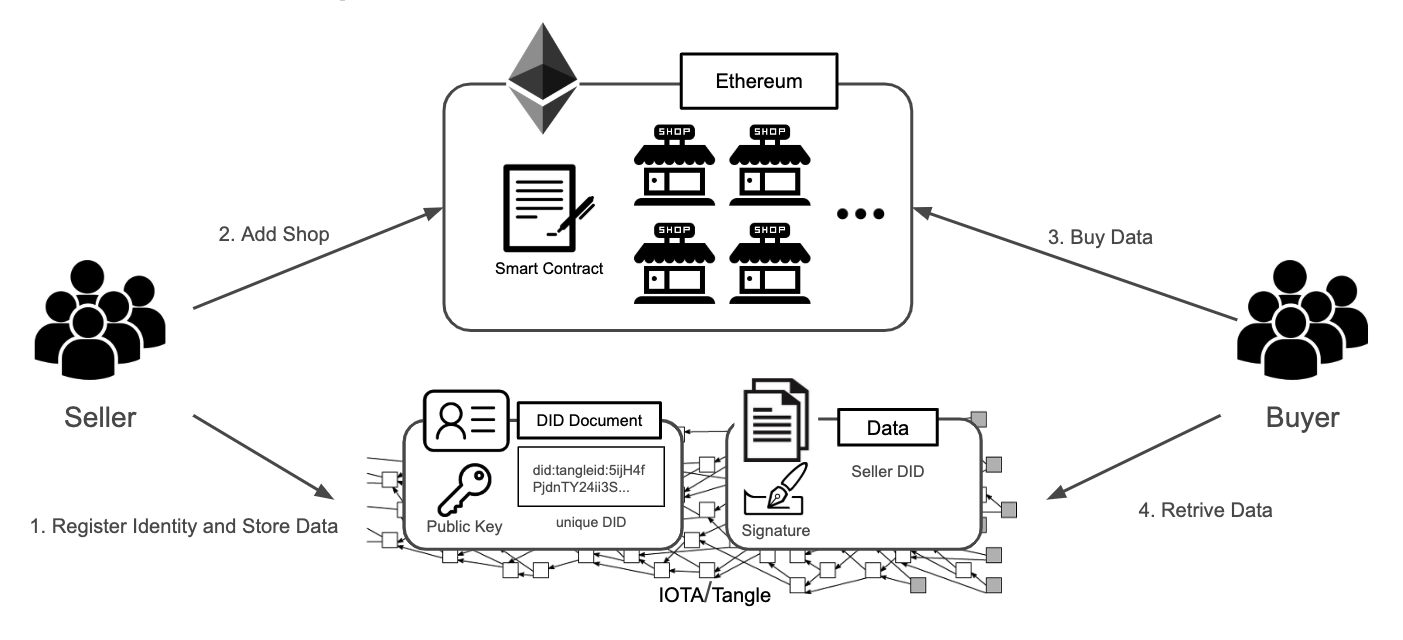
\includegraphics[width=0.5\textwidth]{airbox}
    \caption{IoT-enabled personal air quality assistant.}
    \label{fig:airbox}
\end{figure}

\section{\normalsize\textbf{Related Work}}
The economic value of huge amount of data emerges, several researchers have started to explore the design of data marketplace. The Third Party Auditors (TPAs)-based frameworks is far from being satisfactory due to the unstandardize data format and dynamic nature of IoT data. Therefore a decentralized data integrity validation and trading process has been proposed recent years, and blockchain is considered a solution.

Data Integrity as a Service (DIaaS) is a blockchain based framework for data integrity proposed by Liu et al.\cite{DIaas} which is a Cloud Server Service (CSS) allows both data provider and consumer to validate data integrity by comparing hashes on Ethereum smart contract and Cloud Server. Moreover, Ethereum smart contract can also realize the purchase agreement, including authoriziation and the penalization. However, the architecture of DIaaS needs highly trust on CSS, if CSS is malicious or crashed, that will cause losses to both providers and consumers. Also, the performance analysis shows that IoT devices have low efficiency interacting with Etheruem due to the time-consuming Proof-of-Work(PoW) process.

By solving the inefficiency of the Blockchain, \textbf{IOTA}\cite{IOTAwhitepaper} is a cryptocurrency for the IoT industry based on a revolutionary distributed ledger technology, the \textbf{Tangle}, which enables zero-transaction. On top of that, \textbf{Masked Authenticated Messaging(MAM)}\cite{MAM}, a second layer data communication protocol which allows to emit and access an encrypted data stream over the Tangle where privacy and integrity meet.

On the basis of the Tangle and MAM, IOTA foundation proposed a decentralized Data Marketplace\cite{IOTADataMarket} which is suitable for IoT streaming data that not only allows data providers to put data on Tangle without any trusted cloud services, but also allow providers and consumers to trade on Tangle and protect privacy and assure data integrity from source with MAM. Nevertheless, the platform design is centralized, new devices require manual approval from IOTA team to be visible in the marketplace. Also, interacting with Tangle is still the bottleneck for low-level devices especially in an unstable network or electricity environment.

A different framework design proposed by Gupta, S.Kanhere and Jurdak\cite{3tierDataMarket} could reduce the burden of low-level devices as mentioned. The infrastructure is a 3-tier decentralized data marketplace architectural design with Ethereum smart contract which consists of provider, consumer and broker. Where broker is a highly resourced and trustless device that will facilitate the trading of data between the consumer and providers. However, the data integrity and authentication of each participant are still future work.

The sustainability of IoT economic system is under discussion by Dusit Niyato et al.\cite{UtilityStruct}. They evaluated the utility structure of data trading and presented game theory model with the utility structure which provides a way to find out the Nash Equilibrium. The existence of Nash Equilibrium can help us to determine if the policy of the decentralized data marketplace can ensure a sustainable system. However, few things didn't be mentioned in their work including refund and subscription economy.

The previous work proposed different solution to specific issues of data marketplace. In this paper, we proposed an  overall design of decentralized data marketplace that takes care of data integrity and trading procedure such as buyout and subsciption on distributed ledger.

\section{\normalsize\textbf{System Architecture}}
Our proposed data marketplace framework is a 3-tier decentralized architecture with a registrar who is responsible for marketplace registration in order to put participants' information on distributed ledgers for validation, brokers who interact between data providers and consumers, including data uploading, product metadata generation and trading process, data providers who upload data, and data consumers who search for interested products and issue a new trade.

\subsection{Participants}
There are four major roles in the decentralized data marketplace (Figure \ref{fig:system_design}).

\subsubsection{Registrar}
The registrar is responsible for creating a Registration Contract, which maintains a lookup table of participants, and has the authority to control the participant lists of the decentralized data marketplace.

\subsubsection{Data Provider}
Data providers, who generate and preserve streaming data, are willing to sell streaming data to consumers. They can launch the product on the decentralized data marketplace and receive subscription fees from consumers, which can be used to improve the quantity and accuracy of their device or service.

\subsubsection{Consumer}
Consumers aspire to obtain streaming data to promote the value of their service. However, it is a big challenge for most consumers to collect the desired data by themselves. So they look forward to purchasing the streaming data from data providers.

\subsubsection{Broker}
Brokers represent data providers and consumers to do computing tasks in the DLT (Distributed Ledger Technology) since brokers are expected to have high computing power. Once a data provider wants to launch a new product, the broker is requested to deal with the trading process and upload the provider’s data streams to the MAM channel. For each products, brokerage fees will be charged by the broker.

\begin{figure}[h]
    \centering
    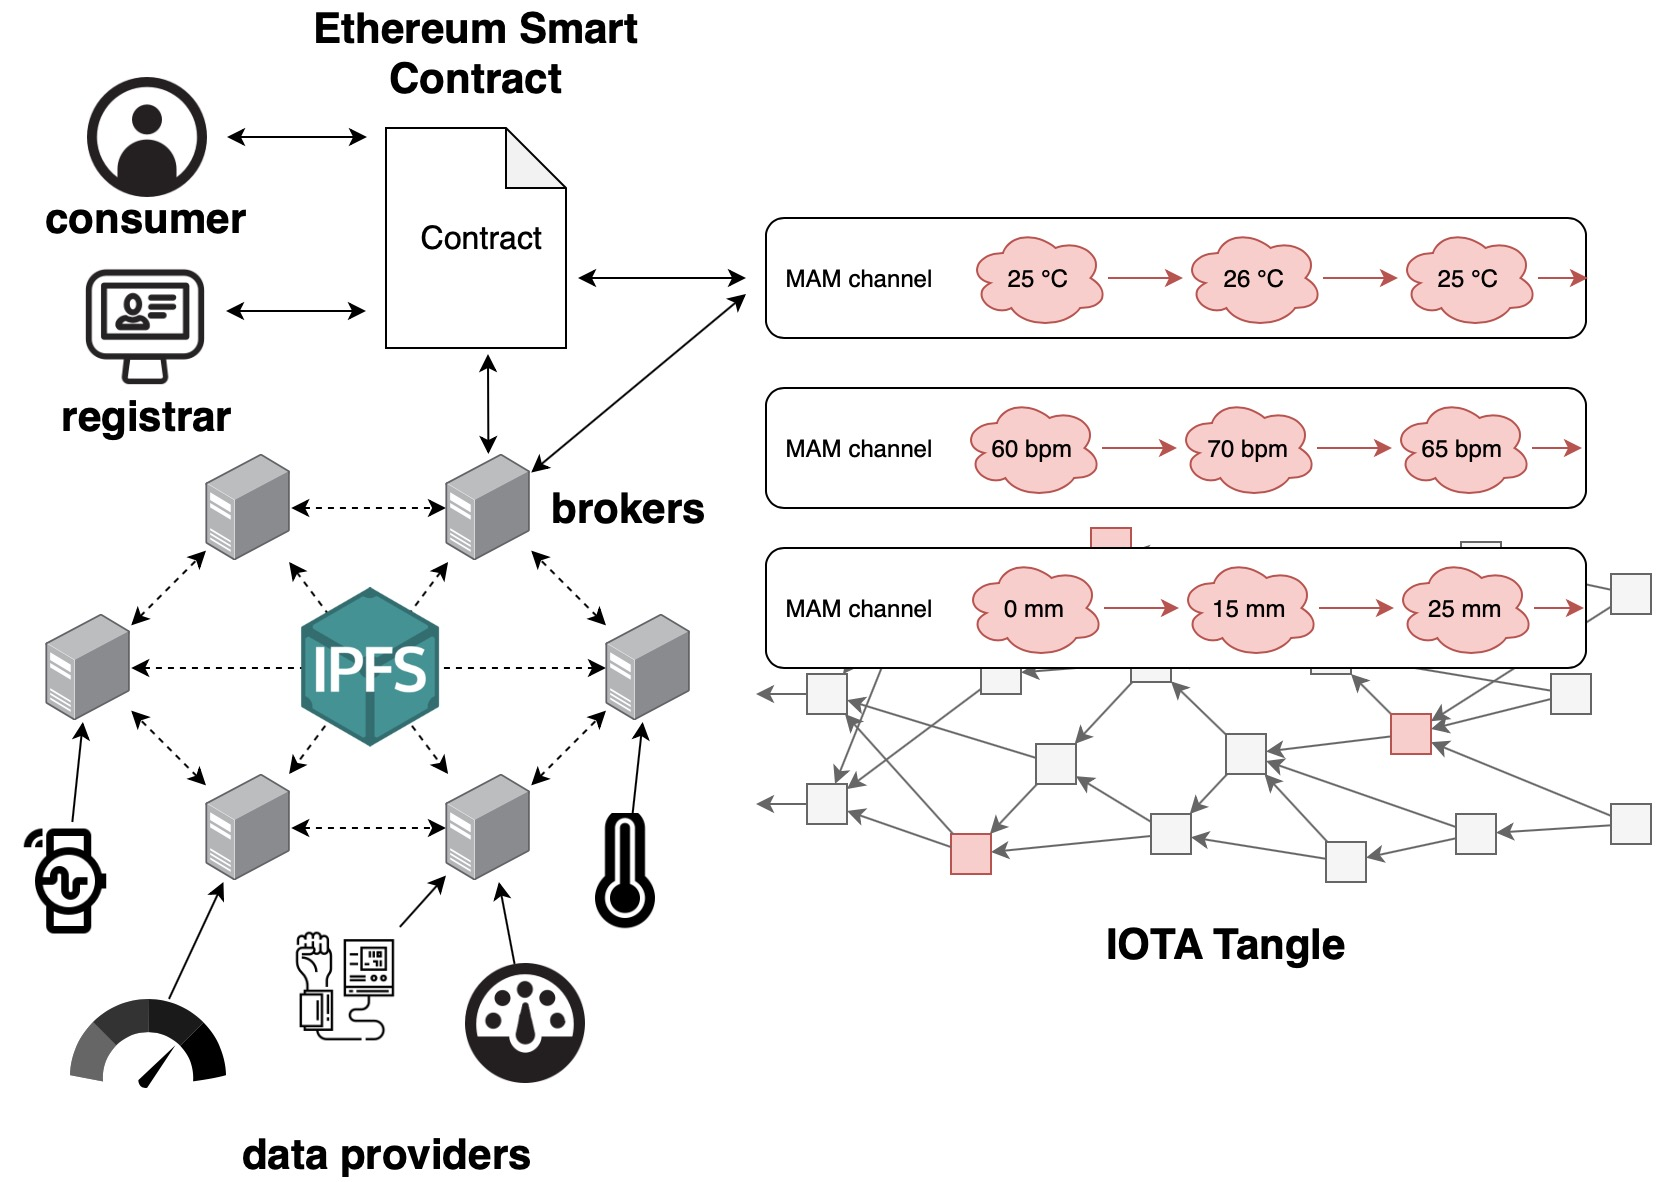
\includegraphics[width=0.4\textwidth]{system_design}
    \caption{System Design.}
    \label{fig:system_design}
\end{figure}

\subsection{Component}
\subsubsection{Masked Authenticated Messaging}
IOTA\cite{IOTAwhitepaper} is a feeless and scalable cryptocurrency for the IoT industry based on a the distributed  ledger consists of a directed acyclic graph(DAG) of individual transactions, \textbf{Tangle}. The innovative consensus algorithm allows people to make \textbf{zero-transactions} that one could store information securely within Tangle transactions. Nevertheless, publishing encrypted streaming data to distributed ledgers is still a challenge, which one need to keep the address and session key per message, otherwise attackers could easily issue spam transactions if publishing with the same address.

However, MAM resolves this problem, it is a second layer data communication protocol enables to emit and access an encrypted data stream over Tangle network and ensures data integrity.
It publishes each message to different addresses that each can be derived from the previous one, this forms a MAM channel. Furthermore, a session key can be provided to control the visibility and access to a MAM channel.

\subsubsection{TangleID}
TangleID\cite{TangleID} is a self-soverign identity system based on IOTA that do not require any third-party authority to verify an identity and its digital footprint. In TangleID, the digital footprint is converted into digital assets with the principle of Decentralized Identifiers (DIDs)\cite{DID} defined by W3C, and by putting DID documents on MAM makes TangleID a GDPR-Complianced system. With every participant in data marketplace registers on TangleID, one can easily verify data providers' identity to ensure the data persistency from data sources.

\subsubsection{Ethereum Smart Contract}
Smart contract\cite{smartContract} is a protocol for formulating agreement on blockchain that provides verification and execution of the contract. The code in the smart contract could interact with other contracts, make decisions, store data and transfer cryptocurrency. All conditions and states established in the contract are transparent and with enforcement. The appearance of smart contracts makes trading more flexible, and achieves more complex trading patterns in reality.

\subsubsection{Blind Signature}
Blind signature\cite{blindSig} is a form of digital signature where the message is first "blinded" by a random "blinding factor", then passed to a signer to sign. The resulting message, along with the blinding factor, can be later verified with the signer's public key. In our system design, brokers would perform blind signature during the process of adding new products for data providers, in order to upload the secret key of MAM channel to smart contract without knowing it.

\subsubsection{IPFS}
Inter-Planetary File system(IPFS)\cite{IPFS} is a peer-to-peer network for storing and accessing files, websites, applications, and data in a distributed file system which is not maintained with certain nodes or entities but all IPFS users. In our proposed architecture, brokers are responsible to upload the metadata of products, including title, data provider information and data preview to IPFS in order to provide users with search capabilities to meet the consumers' need.

\section{\normalsize\textbf{Trading Model}}
In the following, we describe the data trading process in detail. To participate a data marketplace, data providers and consumers have to register first. Then data provider can launch its product on the marketplace. Once a product is launched, it is searchable and could be traded afterward. The whole trading and refunding process is defined in smart contracts which are easily traceable and irreversible.

The consumer will pay for the data, only when the data sold by the data provider with high enough quality/accuracy, which we called these data as decent data.
Once the accuracy is lower than a certain threshold, which we called these data as unacceptable data, the consumers would consider this data provider as a low quality data provider, and stop buying data from this data provider.

Refund is a major issue in our research. However, we don't have to take refund as a factor in our game theory model, since in our decentralized data marketplace we use smart contract to store the subscription fee which will be paid to buy the future data. The subscription fee will be paid as new data is transmitted to consumers. In other words, data provider doesn't need to take any procedure to transfer subscription fee from his/her own account to consumers' account. For the same reason, data provider has no responsibility on the refunding processing fee charged by the smart contract as well.

\subsection{Participants Registration}
At the beginning, the registrar creates a Registration Contract (Figure \ref{fig:registration_contract}), which maintains all participants' information, including their DID (Decentralized Identifiers) Documents and public keys. Only one Registration Contract is needed, and everyone can query the participants' public keys. Then some trustworthy brokers who pass procedures for conformity assessment are added to the decentralized data marketplace. Anyone who would like to sell or purchase data may register to become the data providers or consumers. The registrar has the authority to agree with applications. After that, their identities are available in the Registration Contract and launching and trading processes can be started.

\subsection{Launching and Searching Products}

To sell the streaming data, a data provider has to launch a new product on the data marketplace in advance as shown in Figure \ref{fig:launching_product}. The data provider determines a trusted broker and asks the broker to create a new MAM channel and Product Contract. Each product has a Product Contract to record the participants, subscription price brokerage fee, quantity of data and  trading process.

\begin{figure}[h]
	\centering
	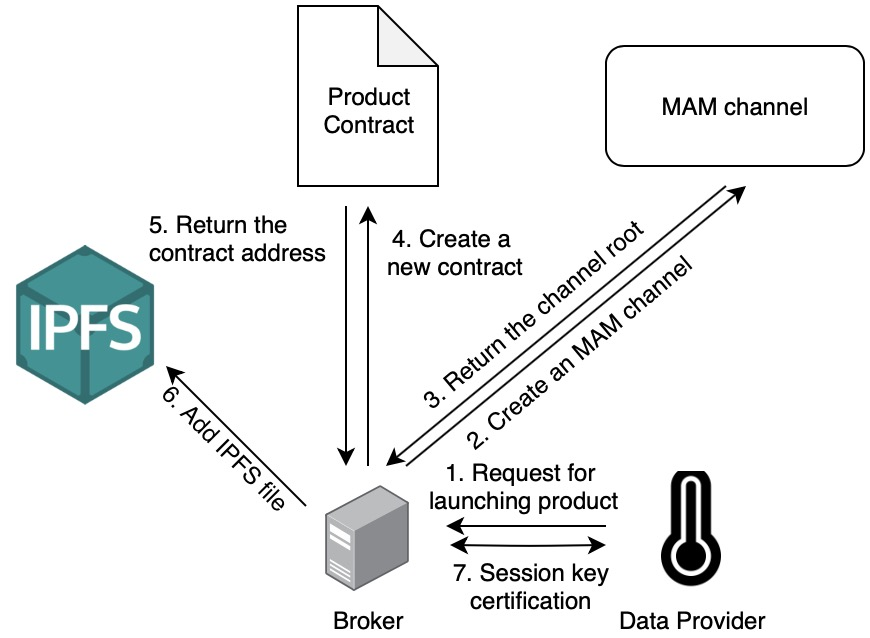
\includegraphics[width=0.4\textwidth]{launching_product}
	\caption{The process of launching a product.}
	\label{fig:launching_product}
\end{figure}

Brokers certify session keys as well. Only one session key can be signed in each product, so data providers can't fake a session key to deceive consumers. However, it is a risk revealing session keys to brokers since contents may be copied by brokers, which causes data providers' loss. Therefore, Blind signature is used to prevent the situation. Figure \ref{fig:key_certification} shows the certification process. When a data provider asks a broker to ceritfy new session key $k$, the data provider uses the broker's public key, which is available in the Registration Contract after the broker's registration, as a blinding factor, and the session key is blinded. Then the data provider sends the blinded session key $Blind(k)$ to the broker. The broker signs the message and returns the signature $Sign(Blind(k))$ to data provider. The data provider removes the blinding factor and obtains the broker's signature of the session key, $Sign(k)$, which is verifiable by consumers.

\begin{figure}[h]
    \centering
    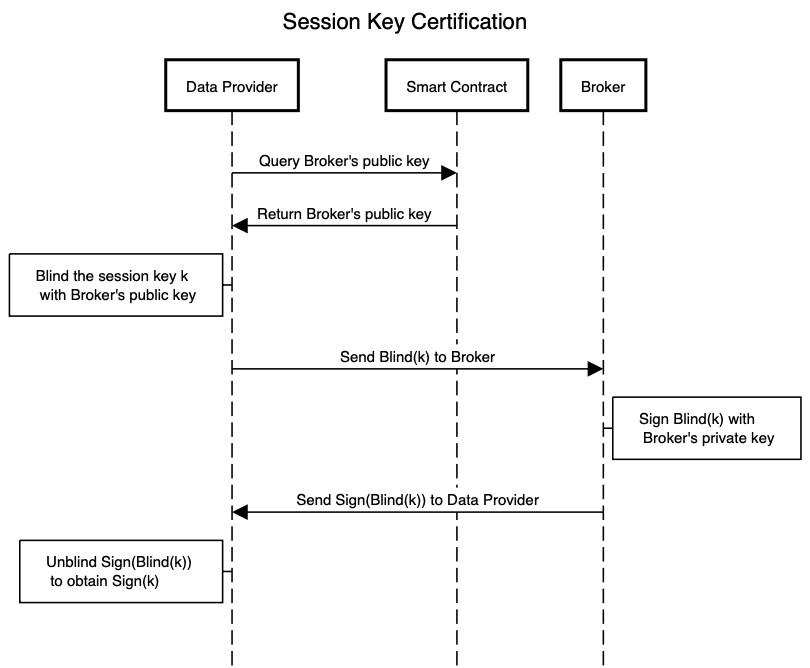
\includegraphics[width=0.5\textwidth]{key_certification}
    \caption{Session key certification process with blind signature.}
    \label{fig:key_certification}
\end{figure}

The contract address and product description will be stored in a file which is uploaded to IPFS. Consumers can search the desired product by keywords or tags. The consumer then evaluates the product and start trading with the data provider if the consumer is interested in subscribing the data.

\subsection{Trading}

\begin{figure}[h]
    \centering
    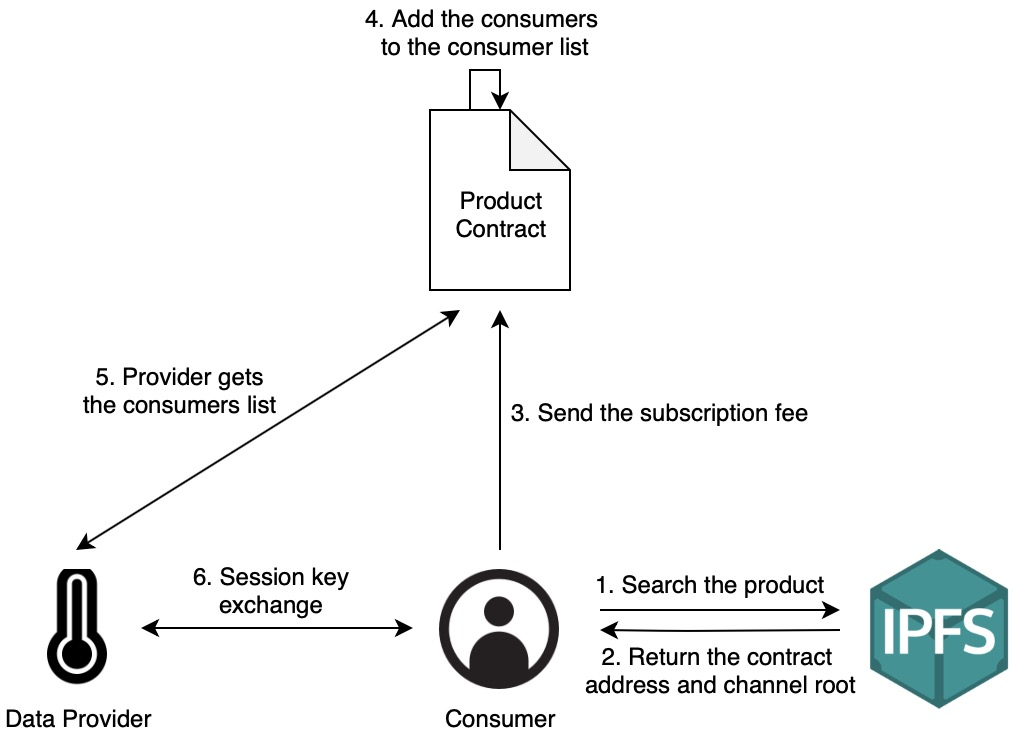
\includegraphics[width=0.4\textwidth]{trading_product}
    \caption{The process of the product trading.}
    \label{fig:trading_product}
\end{figure}

\begin{figure}[h]
    \centering
    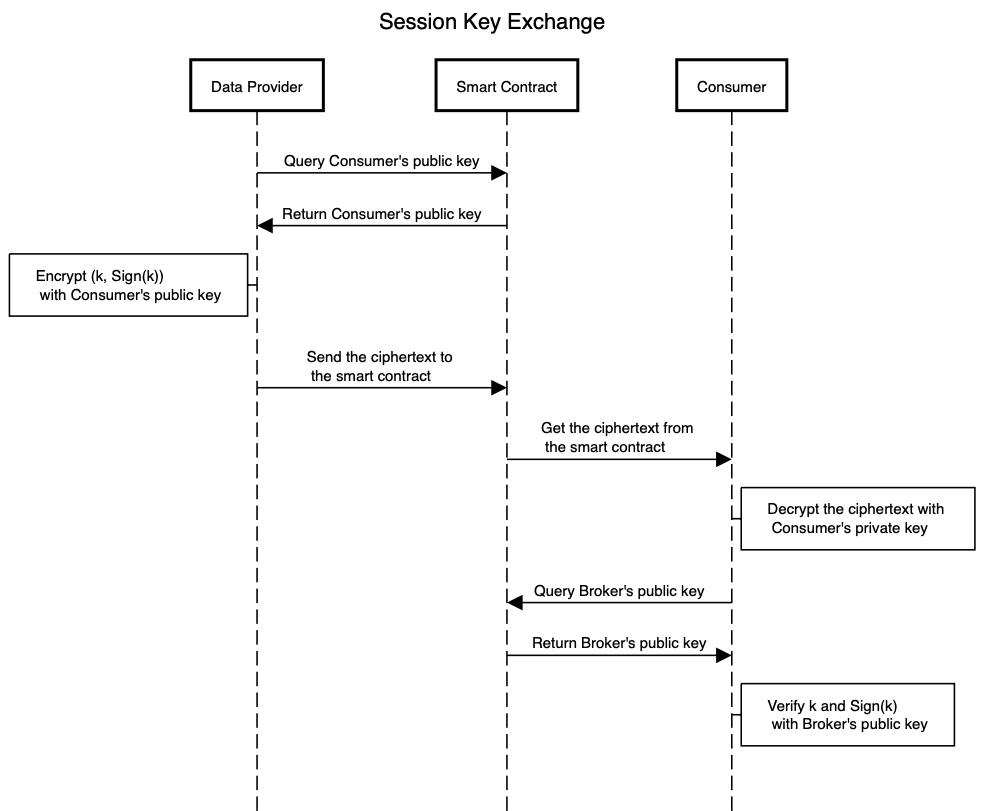
\includegraphics[width=0.5\textwidth]{key_exchange}
    \caption{Session key exchange process between the data provider and consumer.}
    \label{fig:key_exchange}
\end{figure}

The whole trading process is shown in Figure \ref{fig:trading_product}. Once a consumer who wants to subscribe the streaming data pays a subscription fee to the Product Contract, it is added to the consumers list automatically by the smart contract. Next, session key $k$ should be exchanged between data provider and consumers as shown in Figure \ref{fig:key_exchange}.

The data provider can obtain public keys of each consumer from the Registration Contract. For each consumer, the data provider encrypts the session key and broker's signature with the consumer's public key and sends the ciphertext $Encrypt(k + Sign(k))$ to the Product Contract. Consumers listen to the smart contract event which is triggered when the ciphertext is updated, and decrypt the ciphertext to get the session key $k$ and signature $Sign(k)$.

Consumers can obtain the broker's public key on the Registration Contract as well, so they can verify that the signature is valid and the session key is the only one that is certified by the broker. Afterward, encrypted data is uploaded to the MAM channel, and consumers can download and decrypt it with the session key.

\subsection{Refunding}
It is probable that the streaming data sources are delayed or even interrupted after the consumers pay the subscription fee. To protect consumers' right, the subscription fee are not transfered to the data provider until all data is generated and uploaded to the MAM channel. If the expected data is not available, consumers can ask for refunds. We assume that less than half of consumers in the Product Contract are irrational and malicious. Each consumer can vote for refunding at any time. If the ratio of consent votes of refunding is higher than the $threshold$ at the $i$th piece of data, the subscription fee is proportionally transfered to the data provider, broker and every consumer. The subscription fee can be prorated as below:

\begin{equation}
    F_{DataProvider}(i) = N price \frac{i-1}{M} (1-F_{b}) (1-F_{t})
\end{equation}

\begin{equation}
    F_{Broker}(i) = N price \frac{i-1}{M} F_{b} (1-F_{t})
\end{equation}

\begin{equation}
    F_{Consumer}(i) = price \frac{M-i+1}{M} (1-F_{t})
\end{equation}

where $price$  is the subscription price, $M$ is the number of expected data samples, $F_{b}$ is the brokerage fee(\%), $F_{t}$ is the transaction fee of the smart contract(\%), $N$ is the number of consumers in this contract.

To refund or withdraw subscription fee from the smart contract, data provider, broker, and consumer send a transaction to execute the smart contract and are responsible for transaction fee. We assume that only a half of the expected records are uploaded to the MAM channel. For the data provider and broker, they can withdraw a half of total subscription fee from the smart contract and $F_{b}$ \% belongs to the broker while the remaining belongs to the data provider. For consumers, they can get a half refund which should be deducted the transaction fee.

On the other hand, we would consider the situation that one of the consumers requests a refund in our future work. When the consumer is disappointed with the data quality, it may request a refund. Its permit should be cancelled while other consumers are unaffected.

\subsection{Game Theory Evaluation}
Game Theory is a methodology to discuss strategic interaciton among game players. If we can ensure Nash Equilibrium of decentralized data marketplace exists at certain acceptable range, then we can promise the sustainability of decentralized data marketplace. Fan Liang et al\cite{SurveyBigDataPricing} listed several different types of game theory models which are applied on data pricing. To describe the scenario more precisely, we decided to use repeated game to build our game theory model which meets the scenario of subscription economy more.

Figure.\ref{fig:decision_tree} shows the decision tree to depict the the repeated game we used. Each level in this decision tree represents each round of data transmission from data provider to consumers, and the consumers would pay subscription fee, $p_s$, each person. The sum of all the subscription fee pays to data provider is denoted as $P_s$.

\begin{figure} \centering 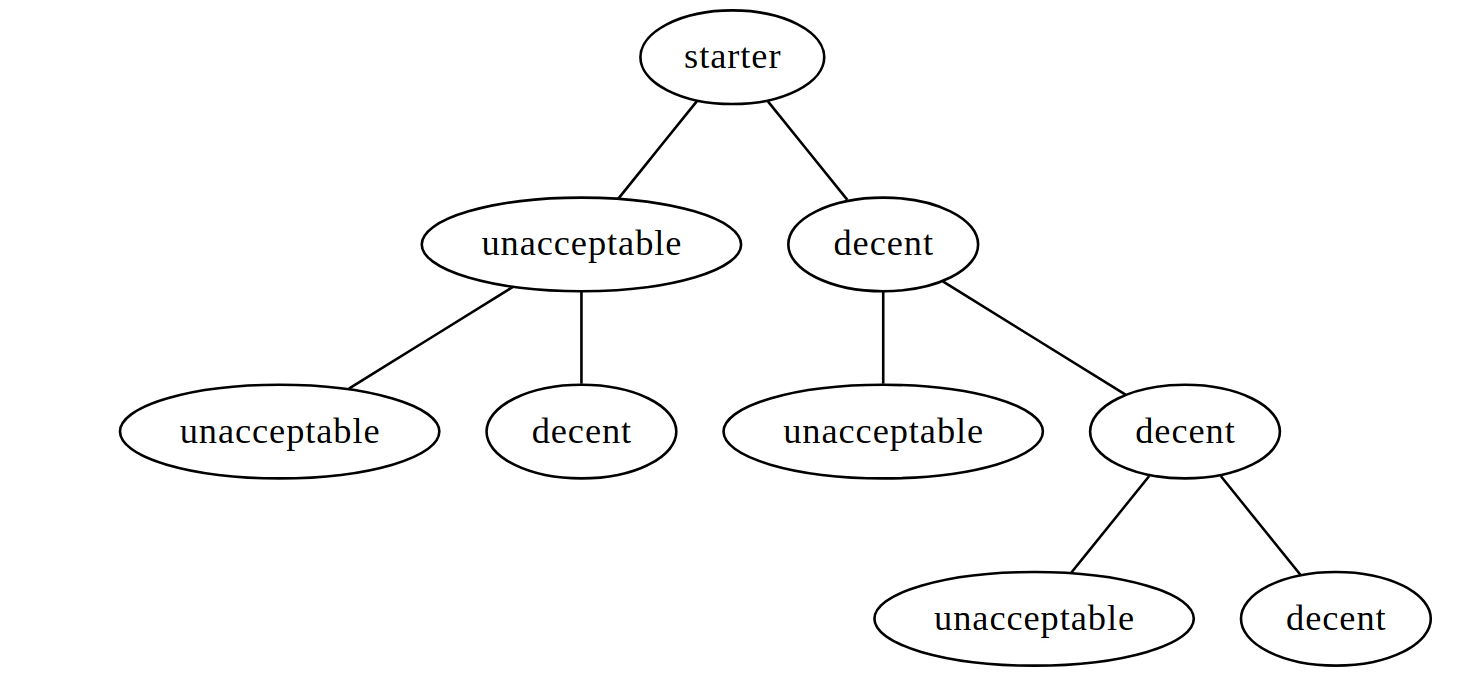
\includegraphics[width=3.3in]{decision_tree} \caption{Decision Tree}
    \label{fig:decision_tree} \end{figure}
For every $n$ round, the data provider would cost $C_{maintain}$ to maintain or enhance the sensors that data provider owns. We call this as a maintain period. Moreover, the value of data and the cost of maintenance will decrease as time pass, so we introduce a discounted factor $\beta$ to depict this phenomena.

We have these following assumptions:
\begin{itemize}
    \item  There is no any other data providers provide the same product in Data Marketplace. Therefore, we can consider each provider's behavior independently. That means this decision tree represent the behavior of only one data provider.
    \item  More than 51\% of consumers are among complete information exchange state. In other words, once one of them launches voting for stopping buying data and refunding, they would succeed in refund voting.
    \item  One of the consumers who has complete information exchange with other 51\% buyers has the ability to examine the data quality. If unacceptably low accuracy data are delivered to consumers, this examiner will spread this information out.
    \item  We assume the number of dishonest consumers is really small, so it can be negleted.
\end{itemize}

Based on the description above, the discounted sum of payoff for our repeated game is
\begin{equation} \label{payoff}
    \sum_{i=0}^{m - 1}{\beta^{in}\cdot [(\sum_{j=0}^{n - 1} \beta^j \cdot P_s) - C_{maintain}]}
\end{equation}

Al-Fagih et al. presented\cite{DataPrice} $P_s$ is sigmoid function of $P_r$, and based on rule of thumb $C_{maintain}$ is about a exponential function of $P_r$. We can substitute $P_s$ and $C_{maintain}$ with $P_r$ into Eq. (\ref{payoff}), then we can find out the Nash Equilibrium of repeated game. We will discuss more in the next section.

\subsubsection{Numerical Example}
To evaluate the behavior of the model we presented, first, we would express the function of $P_s$ and $C_{maintain}$ as function of $P_r$ respectively. Therefore, the sum of subscription fee of all subscriber can be expressed as

\begin{equation} \label{sub_fee}
P_s = R \frac{e^{a (P_r - b)}}{1 + e^{a (P_r - b)}}
\end{equation}

where $a$ and $b$ are tuning factors, and $R$ is the maximun data value.
And we would express the cost of maintenance as

\begin{equation} \label{C_mtn}
C_{maintain} = ce^{P_r - d}
\end{equation}
Where $c$ and $d$ is tuning factor.

Substitute Eq. (\ref{sub_fee}) and Eq. (\ref{C_mtn}) into Eq. (\ref{payoff}). We can derive
\begin{equation} \label{payoff_Pr}
\sum_{i=0}^{m - 1}{\beta^{in}\cdot [(\sum_{j=0}^{n - 1} \beta^j \cdot R \frac{e^{a (P_r - b)}}{1 + e^{a (P_r - b)}}) - ce^{P_r - d}]}
\end{equation}

Let tuning factors $, a = 0.15, b = 50, R = 10000, c = 1, d = 88$, and there is only one maintenance period has happened and one maintenance period consists of 12 rounds which means $m = 1, n = 12$. Based on these parameters, we can plot the payoff function as function of accuracy, $Pr$ which is Figure.\ref{fig:payoff_pic}. The maximun point occurs at $accuracy \approx 92\%$ which we point it out with red dot.
\begin{figure} \centering 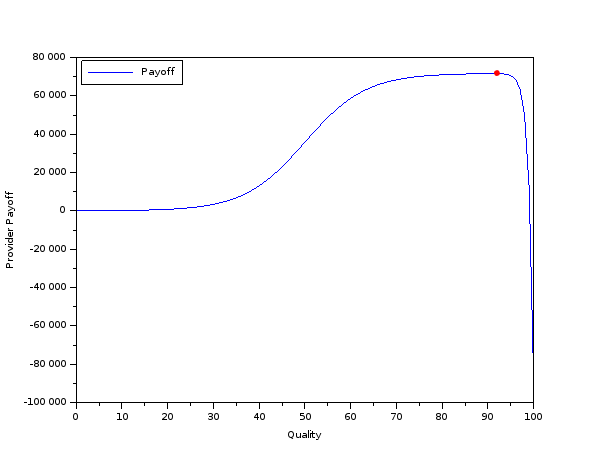
\includegraphics[width=3.3in]{payoff_pic} \caption{Payoff Function}
    \label{fig:payoff_pic} \end{figure}

Figure.\ref{fig:payoff_pic} illustratres the market mechanism of the subscription trading policy we used under the decentralized data marketplace. First, data providers have weak motivation to operate their sensor in low accuracy, since the incentive of low quality data is mush less than moderate quality data. Second the great deficit at high accuracy is mostly drived by the rapid increasing of maintenance cost. Thus, if the maintenance fee to achieve decent data quality is under a fair price range, then data provider will automatically provide data with high enough data quality under our assumptions.

\section{\normalsize\textbf{Future Work}}
%Data Auction
The data auction process is a data trading mechanism and an economically-driven scheme that establishes corresponding prices of data products through bidding process between consumers and providers. While there has been many auction models\cite{BigPicDataMarket} in several areas, only a few of research focus on third-party auction platform. Our proposed decentralized data marketplace protects the privacy of participants which reveals the minimum information for validation and reduces the suspicion of trust to centralized parties or auctioneers. However, the auction process between multiple participants and analyzing potential threats are still critical issues that need to be resolved.

 
% ---- Bibliography ----
\bibliographystyle{IEEEtran}
\bibliography{references}
\end{document}
